\documentclass{beamer}
\usetheme{Copenhagen}
\usecolortheme{orchid}


% Title page details: 
\title{67542 Final Project} 
\author{Yossi R. and Tzahi G.}
\date{August 8, 2022}
%\logo{\large \LaTeX{}}

\newcommand\blfootnote[1]{%
	\begingroup
	\renewcommand\thefootnote{}\footnote{#1}%
	\addtocounter{footnote}{-1}%
	\endgroup
}
\begin{document}
\setbeamertemplate{caption}{\raggedright\insertcaption\par}

\begin{frame}
    \titlepage 
\end{frame}

% Remove logo from the next slides
\logo{}
 
% Outline frame
\begin{frame}{Outline}
    \tableofcontents
\end{frame}

%%%%%%%%%%%%%%%%%%%%%%%%%%%%%%%%%%%%%%%%%%%%%%%%%%%%%%%%%%%%%%%%%%%%%%%%%%%%%%%
\section{Overview}

\begin{frame}{Summary}
\begin{itemize}
\item \textbf{Goal}: Perform metric reconstruction of a scene 

\begin{itemize}
	\item without having camera calibration
	\item using knowledge of  \textit{parallel lines} and \textit{orthogonality} in scene
\end{itemize}

\end{itemize}
\end{frame}

\begin{frame}{Example}
	\begin{figure}
		\centering
		\includegraphics[width=.60\textwidth]{../figures/vanishing_lines_living_room_1.png}
		\caption{Vanishing lines in the scene}
		\label{fig:Vanishing lines}
	\end{figure}

\blfootnote{Image from ETH3D "living room" dataset}
\end{frame}

\begin{frame}{Example}
	\begin{figure}
		\centering
		\includegraphics[width=.60\textwidth]{../figures/vanishing_points_living_room_1.png}
		\caption{Corresponding (mutually orthogonal) vanishing points }
		\label{fig:Vanishing points}
	\end{figure}

\end{frame}


%%%%%%%%%%%%%%%%%%%%%%%%%%%%%%%%%%%%%%%%%%%%%%%%%%%%%%%%%%%%%%%%%%%%%%%%%%%%%%%
\section{Theory}

\begin{frame}{Theory: Scene Reconstruction}
Reminder: 
\begin{itemize}
	\item Given 2 views, and no information about the cameras, we can create a 3d reconstruction only up to a projective transformation, known as a \textbf{projective reconstruction}. 
	\item Given the camera calibration(s), we can upgrade the reconstruction to a \textbf{metric/euclidean reconstruction}, meaning angles in the scene are preserved by the reconstruction, and the reconstruction gives the true aspect ratio of the scene.
\end{itemize}

\blfootnote{Detailed in HZ ch. 10.}

\end{frame}


\begin{frame}{Theory: Camera Intrinsics K}
\begin{itemize}
\item The camera calibration matrix $ K $ has \textbf{5 DOF}.
\begin{itemize}
\item Having three of sets of mutually orthogonal vanishing lines provides \textbf{3 constraints}. 
\item Assuming (1) a zero-skew camera and (2) a camera with known aspect ratio ($ \frac{f_x}{f_y} $) adds \textbf{2 more constraints}.
\item So if our assumptions are correct, and our measurements are accurate, we can solve the system accurately!
\end{itemize}
\end{itemize}
\end{frame}

\begin{frame}{Theory: Camera Intrinsics K}

Reminder: In general, $ K $ has 5 DOF.
\[
K = 
\begin{bmatrix}
f_x & s & c_x \\
0 & f_y & c_y \\
0 & 0 & 1 \\
\end{bmatrix}
\]
\end{frame}

\begin{frame}{Theory: Camera Intrinsics K}
	
We assume  \\
(1) Zero-skew: $ s = 0 $  \\
(2) Known aspect ratio. $ \frac{f_x}{f_y} = \alpha $, where $ \alpha $ is known.\\ In our case, we assume $ \alpha=1 $.
 
As shown, the search is reduced to 3 parameters: 
\[
K = 
\begin{bmatrix}
\alpha f_y & 0 & c_x \\
0 & f_y & c_y \\
0 & 0 & 1 \\
\end{bmatrix}
\]
\end{frame}


\begin{frame}{Theory: IAC}
\begin{itemize}
\item The \textbf{Absolute Conic} is a complex conic lying on the plane at infinity, whose relative position is unchanged as a camera moves in space. 
\item Its image, the \textbf{Image of the Absolute Conic (IAC)} denoted as $ \omega $, is therefore constant for fixed intrinsic parameters $ K $.

\end{itemize}
\end{frame}

\begin{frame}{Theory: IAC}
Knowing the Image of the Absolute Conic (IAC) $ \omega $ is equivalent to knowing the calibration $ K $: 
\begin{itemize}
	\item $ \omega = \left( KK^\mathsf{T} \right)^{-1} \Longleftrightarrow  \omega^{-1} = KK^\mathsf{T} $.
    (Result 8.17 in HZ).
	\item  $ \omega^{-1} = KK^\mathsf{T} $ is symmetric and PD, so the Cholesky decomposition exists: 
	$\boxed{ K = cholesky\left(\omega^{-1}\right) }$
\end{itemize}
\blfootnote{See HZ pp.210, 275}
	
\end{frame}

\begin{frame}{Theory: Scene constraints on the IAC}

\begin{itemize}

\item Two image points $ u $ and $ v $ corresponding to orthogonal scene directions satisfy
\[
{u}^\mathsf{T} \omega v = 0
\]

\item Therefore, 3 mutually orthogonal vanishing points provide 3 linear constraints on $ \omega $. Combining this with the other 2 equations above provides a linear system of equations with a unique solution for $ \omega $. \\

\end{itemize}

\blfootnote{HZ pp.210 eq 8.10}
\end{frame}

\begin{frame}{Theory: Solving for $ \omega $}


Represent $ \omega $ as homogeneous 6-vector $ \textbf{w} = (w_1, w_2, ..., w_6) $,
where 
\[
\omega = 
\begin{bmatrix}
w_1 & w_2 & w_4 \\
w_2 & w_3 & w_5 \\
w_4 & w_5 & w_6 \\
\end{bmatrix}
\]
\end{frame} 

\begin{frame}{Theory: Solving for $ \omega $: orthogonality}
\begin{block}{Orthogonality constraint}
Let two orthogonal vanishing points be $ u = (u_1, u_2, u_3) ^\mathsf{T} $ and $ v = (v_1, v_2, v_3) ^\mathsf{T} $. Then

\[
\begin{bmatrix}
u_1, u_2, u_3
\end{bmatrix}
\begin{bmatrix}
w_1 & w_2 & w_4 \\
w_2 & w_3 & w_5 \\
w_4 & w_5 & w_6 \\
\end{bmatrix}
\begin{bmatrix}
v_1 \\
v_2 \\
v_3
\end{bmatrix}
= 0
\]

which yields the equation
\[ (v_1 u_1 , v_1 u_2 + v_2 u_1 , v_2u_2, v_1 u_3 + v_3 u_1 , v_2 u_3 + v_3 u_2, v_3 u_3) \textbf{w} = 0
\]
\end{block}
We have 3 such equations.
\blfootnote{HZ pp.225}

\end{frame}	

\begin{frame}{Theory: Solving for $ \omega $: zero-skew and square pixels}

For zero-skew, $\omega_{12} = \omega_{21} = 0 $, i.e. $ w_2 = 0 $:

\[
(0, 1, 0, 0, 0, 0) \textbf{w} = 0 
\]

And for square pixels, $ \omega_{11} = \omega_{22} $ i.e.	$ w_1  = w_3 $

\[
(1, 0, -1, 0, 0, 0) \textbf{w} = 0 
\]

\end{frame}


\begin{frame}{Theory }
After solving for $ \omega $, we can compute $ K $ using the above result.
\[
K = cholesky\left(\omega^{-1}\right)
\]
\end{frame}

%%%%%%%%%%%%%%%%%%%%%%%%%%%%%%%%%%%%%%%%%%%%%%%%%%%%%%%%%%%%%%%%%%%%%%%%%%%%%%%
\section{Implementation \& Results}
\begin{frame}{The Algorithm}

\begin{block}{Algorithm}
\textbf{Input:} 2 images. \textbf{Output: }Sparse reconstruction of scene.
\begin{enumerate}
    \item Pre-processing: Manually label 3 sets of mutually orthogonal vanishing lines in each of the images. Then, for each image compute $ \omega_1, K_1 $, and $ \omega_2, K_2 $ (from above).
	\item Find putative matches using SIFT.
	\item Run RANSAC to estimate fundamental matrix $ F $ and select inlier matches.
	\item Convert F to essential matrix $ E $: $ E = {K_2}^\mathsf{T} F K_1 $.
	\item From $ E $, recover relative pose matrices $ M_1 $ and $ M_2 $, then compute $ P_1 = K_1 M_1 $ and $ P_2 = K_2 M_2 $
	\item Triangulate inlier matched points using camera matrices $ P_1 $ and $ P_2 $ to create a sparse reconstruction of the scene.
\end{enumerate}
\end{block}
\end{frame}  

\begin{frame}{Dataset}
	We used the ETH3D dataset, since it contains undistorted images, with calibration information. This was useful for debugging, and to compare to a ground truth.
\begin{figure}
\centering
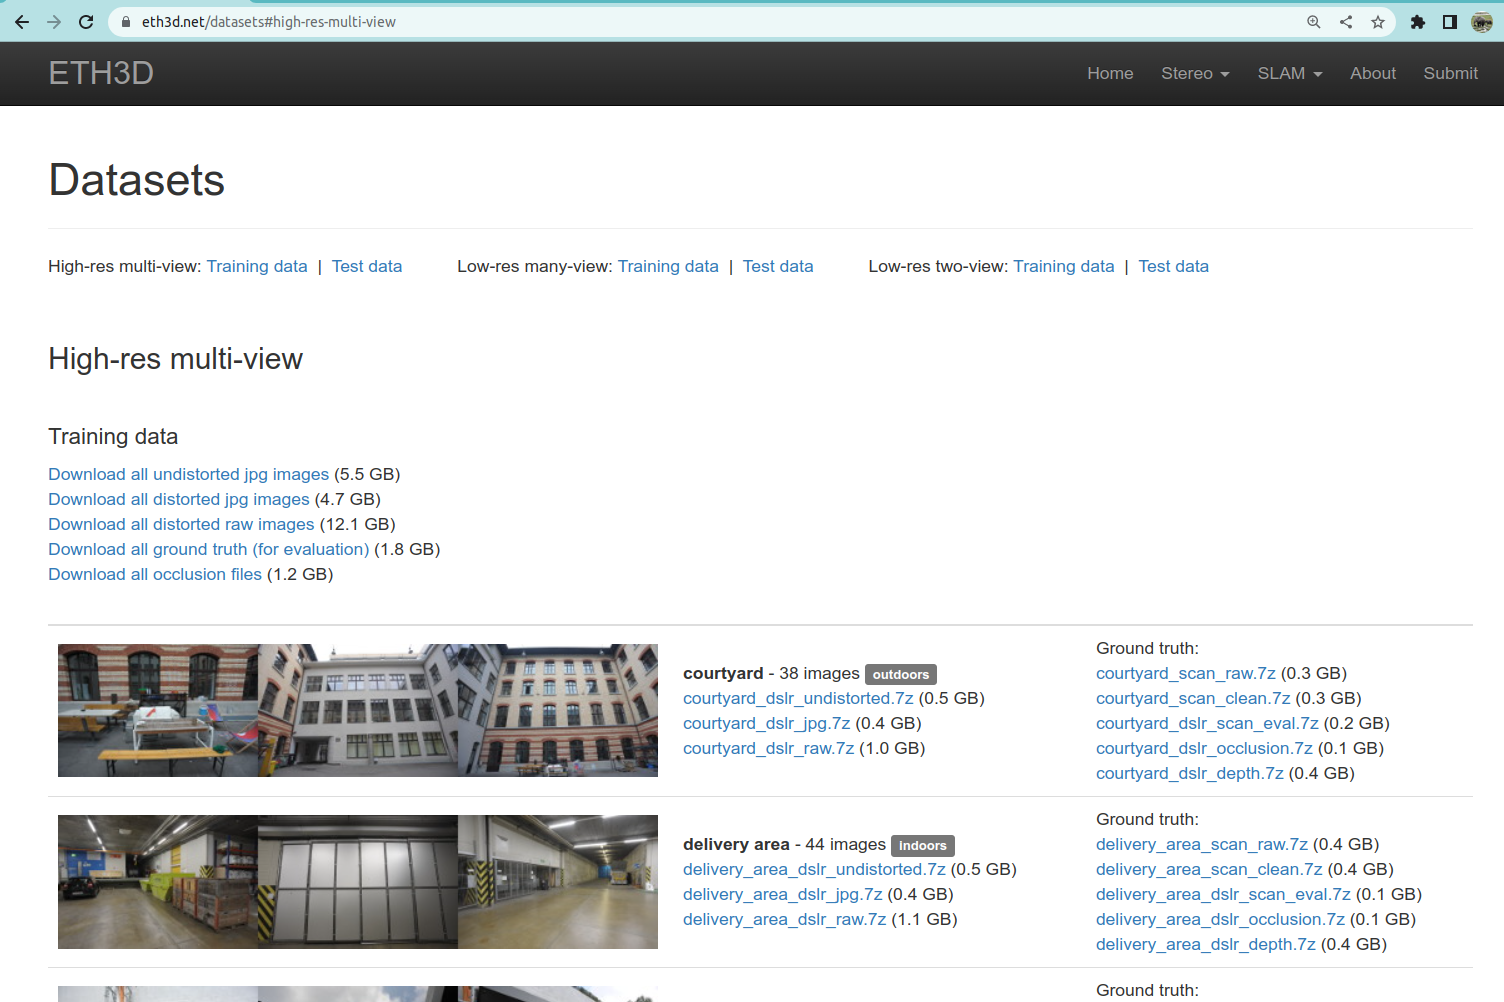
\includegraphics[width=.60\textwidth]{./eth3d_screenshot.png}
\label{fig:ETH3D Dataset}
\end{figure}
\end{frame}	


\begin{frame}{Results}
Example reconstruction
\end{frame}

{
	\setbeamertemplate{navigation symbols}{}
	\setbeamertemplate{background canvas}{\includegraphics[width = \paperwidth]{../figures/vanishing_lines_living_room_1.png}}
	\begin{frame}[plain]
	\end{frame}
}

\begin{frame}{Results}
\[
K_{GT} = 
\begin{bmatrix}
3422.9  &   0.  & 3111.07 \\
0.   & 3421.53 & 2055.06\\
0.    & 0. &     1.  \\
\end{bmatrix}
\]
\[
K_{1} = 
\begin{bmatrix}
3432.374   & 0.    & 3139.894\\
0. & 3432.374 & 2021.478\\
0.    & 0. &     1.  \\
\end{bmatrix}
\]
\end{frame}

{
	\setbeamertemplate{navigation symbols}{}
	\setbeamertemplate{background canvas}{\includegraphics[width = \paperwidth]{../figures/vanishing_lines_living_room_2.png}}
	\begin{frame}[plain]
	\end{frame}
}

\begin{frame}{Results}
	\[
	K_{GT} = 
	\begin{bmatrix}
	3422.9  &   0.  & 3111.07 \\
	0.   & 3421.53 & 2055.06\\
	0.    & 0. &     1.  \\
	\end{bmatrix}
	\]
	\[
	K_{2} = 
	\begin{bmatrix}
	
	3502.965 & 0.  &  3219.078 \\
	0. &  3502.965 & 2008.834 \\
	0.    & 0. &     1.  \\
	\end{bmatrix}
	\]
\end{frame}


{
\setbeamertemplate{navigation symbols}{}
\setbeamertemplate{background canvas}{\includegraphics[width = \paperwidth]{../figures/living_room_reconstruction_1.png}}
\begin{frame}[plain]
\end{frame}
}
{
	\setbeamertemplate{navigation symbols}{}
	\setbeamertemplate{background canvas}{\includegraphics[width = \paperwidth]{../figures/living_room_reconstruction_2.png}}
	\begin{frame}[plain]
	\end{frame}
}
{
	\setbeamertemplate{navigation symbols}{}
	\setbeamertemplate{background canvas}{\includegraphics[width = \paperwidth]{../figures/living_room_reconstruction_3.png}}
	\begin{frame}[plain]
	\end{frame}
}
{
	\setbeamertemplate{navigation symbols}{}
	\setbeamertemplate{background canvas}{\includegraphics[width = \paperwidth]{../figures/living_room_reconstruction_4.png}}
	\begin{frame}[plain]
	\end{frame}
}
{
	\setbeamertemplate{navigation symbols}{}
	\setbeamertemplate{background canvas}{\includegraphics[width = \paperwidth]{../figures/living_room_reconstruction_5.png}}
	\begin{frame}[plain]
	\end{frame}
}
{
	\setbeamertemplate{navigation symbols}{}
	\setbeamertemplate{background canvas}{\includegraphics[width = \paperwidth]{../figures/living_room_reconstruction_6.png}}
	\begin{frame}[plain]
	\end{frame}
}
{
	\setbeamertemplate{navigatio	n symbols}{}
	\setbeamertemplate{background canvas}{\includegraphics[width = \paperwidth]{../figures/living_room_reconstruction_7.png}}
	\begin{frame}[plain]
	\end{frame}
}
{
	\setbeamertemplate{navigation symbols}{}
	\setbeamertemplate{background canvas}{\includegraphics[width = \paperwidth]{../figures/living_room_reconstruction_8.png}}
	\begin{frame}[plain]
	\end{frame}
}
{
	\setbeamertemplate{navigation symbols}{}
	\setbeamertemplate{background canvas}{\includegraphics[width = \paperwidth]{../figures/living_room_reconstruction_9.png}}
	\begin{frame}[plain]
	\end{frame}
}


%%%%%%%%%%%%%%%
{
	\setbeamertemplate{navigation symbols}{}
	\setbeamertemplate{background canvas}{\includegraphics[width = \paperwidth]{../figures/vanishing_lines_observatory_1.png}}
	\begin{frame}[plain]
	\end{frame}
}
\begin{frame}{Results}
	\[
	K_{GT} = 
	\begin{bmatrix}
	3438.51 &   0. &  3121.21 \\
	0. &  3437.06 & 2070.97 \\
	0. &     0.   &   1.  \\
	\end{bmatrix}
	\]
	\[
	K_{1} = 
	\begin{bmatrix}	
    3454.96 &   0. &   3256.888 \\
    0. &     3454.96 & 2029.508 \\
	0.    & 0. &     1.  \\
	\end{bmatrix}
	\]
\end{frame}
{
	\setbeamertemplate{navigation symbols}{}
	\setbeamertemplate{background canvas}{\includegraphics[width = \paperwidth]{../figures/vanishing_lines_observatory_2.png}}
	\begin{frame}[plain]
	\end{frame}
}

\begin{frame}{Results}
	\[
	K_{GT} = 
	\begin{bmatrix}
	3438.51 &   0. &  3121.21 \\
	0. &  3437.06 & 2070.97 \\
	0. &     0.   &   1.  \\
	\end{bmatrix}
	\]
	\[
	K_{2} = 
	\begin{bmatrix}	
	3487.275     & 0.  &   3236.624 \\
	0. &   3487.275 & 2058.119 \\
	0.    & 0. &     1.  \\
	\end{bmatrix}
	\]
\end{frame}

{
	\setbeamertemplate{navigation symbols}{}
	\setbeamertemplate{background canvas}{\includegraphics[width = \paperwidth]{../figures/observatory_reconstruction_1.png}}
	\begin{frame}[plain]
	\end{frame}
}
{
	\setbeamertemplate{navigation symbols}{}
	\setbeamertemplate{background canvas}{\includegraphics[width = \paperwidth]{../figures/observatory_reconstruction_2.png}}
	\begin{frame}[plain]
	\end{frame}
}
{
	\setbeamertemplate{navigation symbols}{}
	\setbeamertemplate{background canvas}{\includegraphics[width = \paperwidth]{../figures/observatory_reconstruction_3.png}}
	\begin{frame}[plain]
	\end{frame}
}
{
	\setbeamertemplate{navigation symbols}{}
	\setbeamertemplate{background canvas}{\includegraphics[width = \paperwidth]{../figures/observatory_reconstruction_4.png}}
	\begin{frame}[plain]
	\end{frame}
}
{
	\setbeamertemplate{navigation symbols}{}
	\setbeamertemplate{background canvas}{\includegraphics[width = \paperwidth]{../figures/observatory_reconstruction_5.png}}
	\begin{frame}[plain]
	\end{frame}
}
{
	\setbeamertemplate{navigation symbols}{}
	\setbeamertemplate{background canvas}{\includegraphics[width = \paperwidth]{../figures/observatory_reconstruction_6.png}}
	\begin{frame}[plain]
	\end{frame}
}
{
	\setbeamertemplate{navigation symbols}{}
	\setbeamertemplate{background canvas}{\includegraphics[width = \paperwidth]{../figures/observatory_reconstruction_7.png}}
	\begin{frame}[plain]
	\end{frame}
}
{
	\setbeamertemplate{navigation symbols}{}
	\setbeamertemplate{background canvas}{\includegraphics[width = \paperwidth]{../figures/observatory_reconstruction_8.png}}
	\begin{frame}[plain]
	\end{frame}
}

\begin{frame}{Limitations}

\begin{itemize}
\item The obvious: only works on scenes with easily identifiable parallel lines, and three mutually orthogonal vanishing points.
\item Sensitive to accuracy in measuring parallel lines, currently done manually.
\item Assumes a linear camera model (e.g. no radial distortion).
\item Degenerate case: parallel scene lines are parallel in image.
\end{itemize}

\end{frame}  

\begin{frame}{Future Work}
\begin{itemize}
\item Detect parallel lines automatically. Can remove orthogonality requirement and instead use knowledge of identical cameras to create metric reconstruction.
\item Detect right angles automatically (deep learning methods?)

\end{itemize}
\end{frame}


\end{document}
